% Figure: discriminate / generate / inverse design pose three different questions
% about one and the same set of objects.  Design width ~168mm.
\documentclass[border=0pt]{standalone}
\usepackage{amsmath,amssymb}
% Shared visual language for the figures of the book.
% Every figure in this directory loads this file so the chapter reads as one system.
% NOTE: no blank lines are allowed inside \tikzset{...} (a blank line emits \par
% and breaks key scanning).
\NeedsTeXFormat{LaTeX2e}
\ProvidesPackage{figstyle}[2026/10/21 Figure style for Free Energy to LLMs]

\RequirePackage{tikz}
\usetikzlibrary{arrows.meta,positioning,calc,fit,shapes.geometric,shapes.misc,%
  backgrounds,matrix,decorations.pathreplacing,decorations.markings,patterns.meta}

% ---------------------------------------------------------------- palette
% Same values as book/preamble/style.tex, prefixed with F.
\definecolor{FNavy}{HTML}{14324A}
\definecolor{FTeal}{HTML}{0E7490}
\definecolor{FSky}{HTML}{E7F5F8}
\definecolor{FOrange}{HTML}{D97706}
\definecolor{FAmber}{HTML}{FFF3D6}
\definecolor{FInk}{HTML}{1F2937}
\definecolor{FSlate}{HTML}{64748B}
\definecolor{FMist}{HTML}{F5F7FA}
\definecolor{FRose}{HTML}{9F1239}
\definecolor{FRoseMist}{HTML}{FFF1F2}

% ---------------------------------------------------------------- semantics
% Teal   = probability / model / data object
% Orange = training objective, cost, or the quantity moved through the system
% Navy   = neutral structure
% Slate  = secondary label or metadata
% Rose   = failure mode, hazard, masked-out region
\tikzset{
  % Lay figures out in millimetres.  A figure designed 168mm wide is included at
  % \textwidth, so its fonts appear at exactly the size written here.
  every picture/.style={x=1mm,y=1mm,font=\small,line cap=round,line join=round},
  % ---- block styles
  nbase/.style={draw,rounded corners=1.2pt,align=center,inner sep=2.4pt,%
    minimum height=7mm,text=FInk},
  nteal/.style={nbase,draw=FTeal,fill=FSky},
  norange/.style={nbase,draw=FOrange,fill=FAmber},
  nnavy/.style={nbase,draw=FNavy,fill=white},
  nsoft/.style={nbase,draw=FSlate!55,fill=FMist},
  nrose/.style={nbase,draw=FRose,fill=FRoseMist},
  ghost/.style={draw=none,fill=none,align=center,inner sep=1pt},
  plain/.style={draw=none,fill=none,align=center,inner sep=0pt},
  % ---- arrows
  ar/.style={-{Latex[length=1.7mm,width=1.35mm]},draw=FSlate,line width=0.75pt},
  ard/.style={ar,dashed},
  arteal/.style={ar,draw=FTeal},
  arorange/.style={ar,draw=FOrange},
  arrose/.style={ar,draw=FRose},
  thickar/.style={ar,line width=1.2pt},
  % ---- text roles
  ftitle/.style={font=\large\bfseries,text=FNavy,align=center},
  ptitle/.style={font=\small\bfseries,text=FNavy,align=center},
  ptitleo/.style={font=\small\bfseries,text=FOrange,align=center},
  lbl/.style={font=\scriptsize,text=FSlate,align=center,inner sep=1pt},
  lblt/.style={lbl,text=FTeal},
  lblo/.style={lbl,text=FOrange},
  lbln/.style={lbl,text=FNavy},
  lblr/.style={lbl,text=FRose},
  sub/.style={font=\scriptsize,text=FSlate!90,align=center,inner sep=1pt},
  monob/.style={font=\ttfamily\scriptsize,text=FInk,inner sep=1pt},
  mathb/.style={font=\small,text=FInk,inner sep=1pt},
  eqn/.style={font=\scriptsize,inner sep=1.5pt,text=FInk},
  % ---- decorations
  brace/.style={decorate,decoration={brace,amplitude=2.4pt},draw=FSlate,%
    line width=0.6pt},
  bracet/.style={brace,draw=FTeal},
  braceo/.style={brace,draw=FOrange},
  axis/.style={draw=FSlate!55,line width=0.6pt},
  guide/.style={draw=FSlate!45,line width=0.5pt,dashed},
  halolabel/.style={font=\scriptsize,text=FInk,fill=white,fill opacity=0.85,%
    text opacity=1,inner sep=1.4pt,align=center},
}

% Figure title above the drawing, anchored at the figure's top-left.
\newcommand{\figtitle}[2][0]{%
  \node[ftitle,anchor=north west,outer sep=0pt] at (#1,0) {#2};}

% Rounded panel behind a subgroup of nodes.
\newcommand{\figpanel}[3][]{%
  \node[draw=FSlate!35,fill=#3,rounded corners=2pt,inner sep=2.6mm,#1] {#2};}

\endinput

\begin{document}
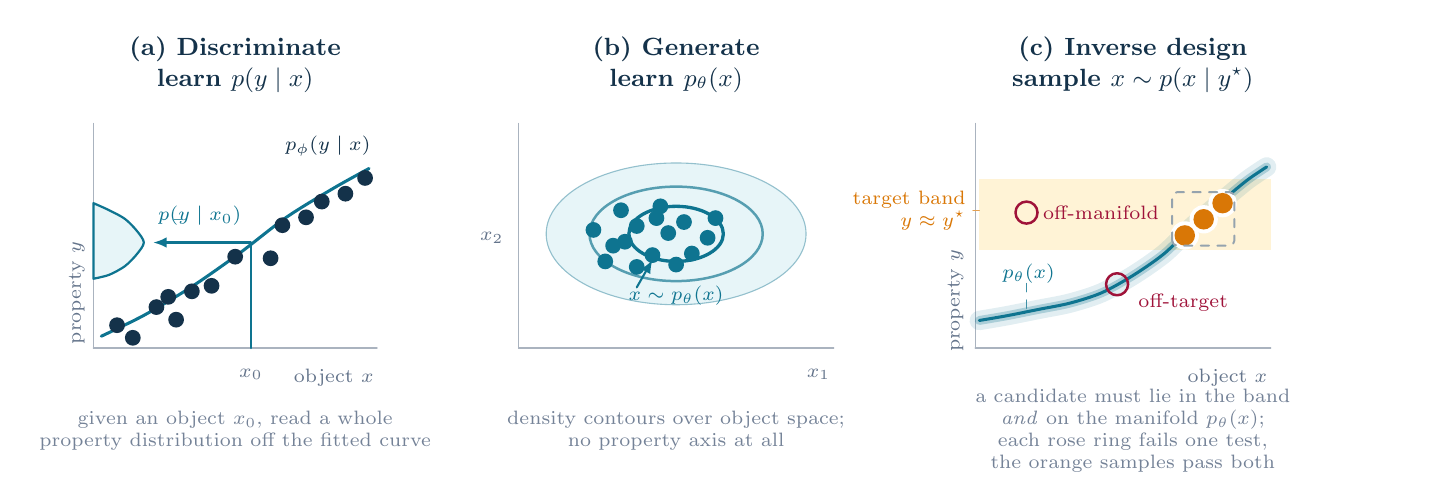
\begin{tikzpicture}
% ---------------------------------------------------------------- (a) discriminate
\node[ptitle] at (30,54) {(a) Discriminate\\learn $p(y\mid x)$};
\draw[axis] (12,18)--(48,18);
\draw[axis] (12,18)--(12,46.5);
\node[lbl,rotate=90] at (9.9,25) {property $y$};
\node[lbl,anchor=north east] at (48,15.8) {object $x$};
\node[lbl,anchor=north] at (32,15.8) {$x_0$};
\draw[draw=FTeal,fill=FSky,line width=0.8pt,smooth] plot coordinates
  {(12,26.8)(14,27.3)(16,28.4)(17.5,29.9)(18.4,31.4)(17.5,32.9)(16,34.4)(14,35.5)(12,36.4)}
  -- cycle;
\draw[FTeal,line width=1.1pt,smooth] plot coordinates
  {(13,19.5)(18.5,22.2)(24.5,25.8)(30.5,30)(36.5,34.6)(42.5,38.3)(47,40.8)};
\foreach \x/\y in {15/20.9,17/19.3,20/23.2,22.5/21.6,24.5/25.2,27/25.9,%
  30/29.6,34.5/29.4,36/33.6,39/34.6,41/36.6,44/37.6,46.5/39.6,21.5/24.5}
  {\fill[FNavy] (\x,\y) circle (1.0);}
\draw[arteal] (32,18)--(32,31.4)--(19.6,31.4);
\node[lblt] at (25.5,34.8) {$p(y\mid x_0)$};
\draw[guide,draw=FTeal!75] (23.2,34.3)--(20.9,34.3);
\node[lbln,anchor=south east] at (47.6,42) {$p_\phi(y\mid x)$};
\node[sub,text width=52mm] at (30,7.5) {given an object $x_0$, read a whole\\property distribution off the fitted curve};
% ---------------------------------------------------------------- (b) generate
\node[ptitle] at (86,54) {(b) Generate\\learn $p_\theta(x)$};
\draw[axis] (66,18)--(106,18);
\draw[axis] (66,18)--(66,46.5);
\node[lbl,anchor=east] at (64.5,32) {$x_2$};
\node[lbl,anchor=north east] at (106,15.8) {$x_1$};
\draw[draw=FTeal!45,fill=FSky] (86,32.5) ellipse (16.5 and 9);
\draw[draw=FTeal!70,line width=0.9pt] (86,32.5) ellipse (11 and 6);
\draw[draw=FTeal,line width=1.2pt] (86,32.5) ellipse (6 and 3.5);
\foreach \x/\y in {78/31,81/33.5,83/29.8,85/32.6,87/34,79/35.5,84/36,88/30,%
  81/28.3,86/28.6,90/32,77/29,91/34.5,75.5/33,83.5/34.5,79.5/31.5}
  {\fill[FTeal] (\x,\y) circle (1.0);}
\node[lblt] at (86,24.6) {$x\sim p_\theta(x)$};
\draw[arteal] (81,25.7)--(83,29.2);
\node[sub,text width=52mm] at (86,7.5) {density contours over object space;\\no property axis at all};
% ------------------------------------------------------------ (c) inverse design
\node[ptitle] at (144,54) {(c) Inverse design\\sample $x\sim p(x\mid y^\star)$};
\draw[axis] (124,18)--(161.5,18);
\draw[axis] (124,18)--(124,46.5);
\node[lbl,rotate=90] at (121.5,24) {property $y$};
\node[lbl,anchor=north east] at (161.5,15.8) {object $x$};
\fill[FAmber] (124.5,30.5) rectangle (161.5,39.5);
\node[lblo,anchor=east,align=right] at (123.2,35.5) {target band\\$y\approx y^\star$};
\draw[guide,draw=FOrange!70] (123.7,35.5)--(124.5,35.5);
\draw[FTeal,line width=7pt,opacity=0.12,smooth] plot coordinates
  {(124.5,21.5)(128,22.1)(132,22.9)(136,23.7)(140,25.0)(144,27.2)(148,30.0)%
   (151.5,33.4)(155,36.4)(158.5,39.3)(161,41.0)};
\draw[FTeal,line width=3.2pt,opacity=0.26,smooth] plot coordinates
  {(124.5,21.5)(128,22.1)(132,22.9)(136,23.7)(140,25.0)(144,27.2)(148,30.0)%
   (151.5,33.4)(155,36.4)(158.5,39.3)(161,41.0)};
\draw[FTeal,line width=1.1pt,smooth] plot coordinates
  {(124.5,21.5)(128,22.1)(132,22.9)(136,23.7)(140,25.0)(144,27.2)(148,30.0)%
   (151.5,33.4)(155,36.4)(158.5,39.3)(161,41.0)};
\node[lblt,anchor=west] at (127,27.4) {$p_\theta(x)$};
\draw[guide,draw=FTeal!80] (130.5,26.2)--(130.5,23.0);
\draw[draw=FRose,line width=0.9pt] (130.5,35.2) circle (1.4);
\node[lblr,anchor=west] at (132.2,35.2) {off-manifold};
\draw[draw=FRose,line width=0.9pt] (142,26.1) circle (1.4);
\node[lblr,anchor=west] at (144.3,23.8) {off-target};
\foreach \x/\y in {150.6/32.3,153/34.35,155.4/36.4}
  {\fill[white] (\x,\y) circle (1.8); \fill[FOrange] (\x,\y) circle (1.3);}
\draw[draw=FNavy!45,dashed,line width=0.7pt,rounded corners=1.8pt]
  (149,31) rectangle (156.9,37.8);
\node[sub,text width=68mm] at (144,7.5) {a candidate must lie in the band \emph{and} on the manifold $p_\theta(x)$;\\%
  each rose ring fails one test, the orange samples pass both};
\end{tikzpicture}
\end{document}
